% Options for packages loaded elsewhere
\PassOptionsToPackage{unicode}{hyperref}
\PassOptionsToPackage{hyphens}{url}
\PassOptionsToPackage{dvipsnames,svgnames,x11names}{xcolor}
%
\documentclass[
  letterpaper,
  DIV=11,
  numbers=noendperiod]{scrreprt}

\usepackage{amsmath,amssymb}
\usepackage{iftex}
\ifPDFTeX
  \usepackage[T1]{fontenc}
  \usepackage[utf8]{inputenc}
  \usepackage{textcomp} % provide euro and other symbols
\else % if luatex or xetex
  \usepackage{unicode-math}
  \defaultfontfeatures{Scale=MatchLowercase}
  \defaultfontfeatures[\rmfamily]{Ligatures=TeX,Scale=1}
\fi
\usepackage{lmodern}
\ifPDFTeX\else  
    % xetex/luatex font selection
\fi
% Use upquote if available, for straight quotes in verbatim environments
\IfFileExists{upquote.sty}{\usepackage{upquote}}{}
\IfFileExists{microtype.sty}{% use microtype if available
  \usepackage[]{microtype}
  \UseMicrotypeSet[protrusion]{basicmath} % disable protrusion for tt fonts
}{}
\makeatletter
\@ifundefined{KOMAClassName}{% if non-KOMA class
  \IfFileExists{parskip.sty}{%
    \usepackage{parskip}
  }{% else
    \setlength{\parindent}{0pt}
    \setlength{\parskip}{6pt plus 2pt minus 1pt}}
}{% if KOMA class
  \KOMAoptions{parskip=half}}
\makeatother
\usepackage{xcolor}
\setlength{\emergencystretch}{3em} % prevent overfull lines
\setcounter{secnumdepth}{5}
% Make \paragraph and \subparagraph free-standing
\ifx\paragraph\undefined\else
  \let\oldparagraph\paragraph
  \renewcommand{\paragraph}[1]{\oldparagraph{#1}\mbox{}}
\fi
\ifx\subparagraph\undefined\else
  \let\oldsubparagraph\subparagraph
  \renewcommand{\subparagraph}[1]{\oldsubparagraph{#1}\mbox{}}
\fi

\usepackage{color}
\usepackage{fancyvrb}
\newcommand{\VerbBar}{|}
\newcommand{\VERB}{\Verb[commandchars=\\\{\}]}
\DefineVerbatimEnvironment{Highlighting}{Verbatim}{commandchars=\\\{\}}
% Add ',fontsize=\small' for more characters per line
\usepackage{framed}
\definecolor{shadecolor}{RGB}{241,243,245}
\newenvironment{Shaded}{\begin{snugshade}}{\end{snugshade}}
\newcommand{\AlertTok}[1]{\textcolor[rgb]{0.68,0.00,0.00}{#1}}
\newcommand{\AnnotationTok}[1]{\textcolor[rgb]{0.37,0.37,0.37}{#1}}
\newcommand{\AttributeTok}[1]{\textcolor[rgb]{0.40,0.45,0.13}{#1}}
\newcommand{\BaseNTok}[1]{\textcolor[rgb]{0.68,0.00,0.00}{#1}}
\newcommand{\BuiltInTok}[1]{\textcolor[rgb]{0.00,0.23,0.31}{#1}}
\newcommand{\CharTok}[1]{\textcolor[rgb]{0.13,0.47,0.30}{#1}}
\newcommand{\CommentTok}[1]{\textcolor[rgb]{0.37,0.37,0.37}{#1}}
\newcommand{\CommentVarTok}[1]{\textcolor[rgb]{0.37,0.37,0.37}{\textit{#1}}}
\newcommand{\ConstantTok}[1]{\textcolor[rgb]{0.56,0.35,0.01}{#1}}
\newcommand{\ControlFlowTok}[1]{\textcolor[rgb]{0.00,0.23,0.31}{#1}}
\newcommand{\DataTypeTok}[1]{\textcolor[rgb]{0.68,0.00,0.00}{#1}}
\newcommand{\DecValTok}[1]{\textcolor[rgb]{0.68,0.00,0.00}{#1}}
\newcommand{\DocumentationTok}[1]{\textcolor[rgb]{0.37,0.37,0.37}{\textit{#1}}}
\newcommand{\ErrorTok}[1]{\textcolor[rgb]{0.68,0.00,0.00}{#1}}
\newcommand{\ExtensionTok}[1]{\textcolor[rgb]{0.00,0.23,0.31}{#1}}
\newcommand{\FloatTok}[1]{\textcolor[rgb]{0.68,0.00,0.00}{#1}}
\newcommand{\FunctionTok}[1]{\textcolor[rgb]{0.28,0.35,0.67}{#1}}
\newcommand{\ImportTok}[1]{\textcolor[rgb]{0.00,0.46,0.62}{#1}}
\newcommand{\InformationTok}[1]{\textcolor[rgb]{0.37,0.37,0.37}{#1}}
\newcommand{\KeywordTok}[1]{\textcolor[rgb]{0.00,0.23,0.31}{#1}}
\newcommand{\NormalTok}[1]{\textcolor[rgb]{0.00,0.23,0.31}{#1}}
\newcommand{\OperatorTok}[1]{\textcolor[rgb]{0.37,0.37,0.37}{#1}}
\newcommand{\OtherTok}[1]{\textcolor[rgb]{0.00,0.23,0.31}{#1}}
\newcommand{\PreprocessorTok}[1]{\textcolor[rgb]{0.68,0.00,0.00}{#1}}
\newcommand{\RegionMarkerTok}[1]{\textcolor[rgb]{0.00,0.23,0.31}{#1}}
\newcommand{\SpecialCharTok}[1]{\textcolor[rgb]{0.37,0.37,0.37}{#1}}
\newcommand{\SpecialStringTok}[1]{\textcolor[rgb]{0.13,0.47,0.30}{#1}}
\newcommand{\StringTok}[1]{\textcolor[rgb]{0.13,0.47,0.30}{#1}}
\newcommand{\VariableTok}[1]{\textcolor[rgb]{0.07,0.07,0.07}{#1}}
\newcommand{\VerbatimStringTok}[1]{\textcolor[rgb]{0.13,0.47,0.30}{#1}}
\newcommand{\WarningTok}[1]{\textcolor[rgb]{0.37,0.37,0.37}{\textit{#1}}}

\providecommand{\tightlist}{%
  \setlength{\itemsep}{0pt}\setlength{\parskip}{0pt}}\usepackage{longtable,booktabs,array}
\usepackage{calc} % for calculating minipage widths
% Correct order of tables after \paragraph or \subparagraph
\usepackage{etoolbox}
\makeatletter
\patchcmd\longtable{\par}{\if@noskipsec\mbox{}\fi\par}{}{}
\makeatother
% Allow footnotes in longtable head/foot
\IfFileExists{footnotehyper.sty}{\usepackage{footnotehyper}}{\usepackage{footnote}}
\makesavenoteenv{longtable}
\usepackage{graphicx}
\makeatletter
\def\maxwidth{\ifdim\Gin@nat@width>\linewidth\linewidth\else\Gin@nat@width\fi}
\def\maxheight{\ifdim\Gin@nat@height>\textheight\textheight\else\Gin@nat@height\fi}
\makeatother
% Scale images if necessary, so that they will not overflow the page
% margins by default, and it is still possible to overwrite the defaults
% using explicit options in \includegraphics[width, height, ...]{}
\setkeys{Gin}{width=\maxwidth,height=\maxheight,keepaspectratio}
% Set default figure placement to htbp
\makeatletter
\def\fps@figure{htbp}
\makeatother
\newlength{\cslhangindent}
\setlength{\cslhangindent}{1.5em}
\newlength{\csllabelwidth}
\setlength{\csllabelwidth}{3em}
\newlength{\cslentryspacingunit} % times entry-spacing
\setlength{\cslentryspacingunit}{\parskip}
\newenvironment{CSLReferences}[2] % #1 hanging-ident, #2 entry spacing
 {% don't indent paragraphs
  \setlength{\parindent}{0pt}
  % turn on hanging indent if param 1 is 1
  \ifodd #1
  \let\oldpar\par
  \def\par{\hangindent=\cslhangindent\oldpar}
  \fi
  % set entry spacing
  \setlength{\parskip}{#2\cslentryspacingunit}
 }%
 {}
\usepackage{calc}
\newcommand{\CSLBlock}[1]{#1\hfill\break}
\newcommand{\CSLLeftMargin}[1]{\parbox[t]{\csllabelwidth}{#1}}
\newcommand{\CSLRightInline}[1]{\parbox[t]{\linewidth - \csllabelwidth}{#1}\break}
\newcommand{\CSLIndent}[1]{\hspace{\cslhangindent}#1}

\usepackage{makeidx}
\makeindex
\KOMAoption{captions}{tableheading}
\makeatletter
\makeatother
\makeatletter
\@ifpackageloaded{bookmark}{}{\usepackage{bookmark}}
\makeatother
\makeatletter
\@ifpackageloaded{caption}{}{\usepackage{caption}}
\AtBeginDocument{%
\ifdefined\contentsname
  \renewcommand*\contentsname{Table of contents}
\else
  \newcommand\contentsname{Table of contents}
\fi
\ifdefined\listfigurename
  \renewcommand*\listfigurename{List of Figures}
\else
  \newcommand\listfigurename{List of Figures}
\fi
\ifdefined\listtablename
  \renewcommand*\listtablename{List of Tables}
\else
  \newcommand\listtablename{List of Tables}
\fi
\ifdefined\figurename
  \renewcommand*\figurename{Figure}
\else
  \newcommand\figurename{Figure}
\fi
\ifdefined\tablename
  \renewcommand*\tablename{Table}
\else
  \newcommand\tablename{Table}
\fi
}
\@ifpackageloaded{float}{}{\usepackage{float}}
\floatstyle{ruled}
\@ifundefined{c@chapter}{\newfloat{codelisting}{h}{lop}}{\newfloat{codelisting}{h}{lop}[chapter]}
\floatname{codelisting}{Listing}
\newcommand*\listoflistings{\listof{codelisting}{List of Listings}}
\makeatother
\makeatletter
\@ifpackageloaded{caption}{}{\usepackage{caption}}
\@ifpackageloaded{subcaption}{}{\usepackage{subcaption}}
\makeatother
\makeatletter
\@ifpackageloaded{tcolorbox}{}{\usepackage[skins,breakable]{tcolorbox}}
\makeatother
\makeatletter
\@ifundefined{shadecolor}{\definecolor{shadecolor}{rgb}{.97, .97, .97}}
\makeatother
\makeatletter
\makeatother
\makeatletter
\makeatother
\ifLuaTeX
  \usepackage{selnolig}  % disable illegal ligatures
\fi
\IfFileExists{bookmark.sty}{\usepackage{bookmark}}{\usepackage{hyperref}}
\IfFileExists{xurl.sty}{\usepackage{xurl}}{} % add URL line breaks if available
\urlstyle{same} % disable monospaced font for URLs
\hypersetup{
  pdftitle={Pollspain},
  pdfauthor={Mikaela De Smedt},
  colorlinks=true,
  linkcolor={blue},
  filecolor={Maroon},
  citecolor={Blue},
  urlcolor={Blue},
  pdfcreator={LaTeX via pandoc}}

\title{Pollspain}
\author{Mikaela De Smedt}
\date{2024-08-25}

\begin{document}
\maketitle
\ifdefined\Shaded\renewenvironment{Shaded}{\begin{tcolorbox}[interior hidden, sharp corners, borderline west={3pt}{0pt}{shadecolor}, breakable, frame hidden, boxrule=0pt, enhanced]}{\end{tcolorbox}}\fi

\renewcommand*\contentsname{Table of contents}
{
\hypersetup{linkcolor=}
\setcounter{tocdepth}{2}
\tableofcontents
}
\bookmarksetup{startatroot}

\hypertarget{package-overview}{%
\chapter*{Package Overview}\label{package-overview}}
\addcontentsline{toc}{chapter}{Package Overview}

\markboth{Package Overview}{Package Overview}

\texttt{pollspain} offers a range of features for its users to work with
Spanish electoral data. Primarily, the centralization of official
electoral data from the Spanish Ministry of the Interior through
\href{https://infoelectoral.interior.gob.es/es/elecciones-celebradas/area-de-descargas/}{Infoelectoral}
(Interior, 2024) through its download, processing and hosting in
\href{https://github.com/mikadsr/Pollspain-data}{Pollspain-data}
(DeSmedt, 2024)the data repository for the package. This makes it so
comprehensive datasets on municipal census information, candidacies,
candidates, polling stations, and CERA data from 1982 until 2023 are
available through the package.

In addition to this, the package also provides ready-made functions for
summarizing and visualizing the information. These functions are
designed to be intuitive and easy to use, enabling users to quickly
generate insights from the data without requiring extensive programming
knowledge.

Lastly, a key feature of the package is the access to electoral survey
data. This allows users to access a collection of public opinion polling
results and perform analysis such as polling error and house effects on
them.

Overall, \texttt{pollspain} combines data sourcing, processing and
analysis into a single package that empowers users to engage deeply with
Spanish electoral data.

\bookmarksetup{startatroot}

\hypertarget{introduction}{%
\chapter{Introduction}\label{introduction}}

\hypertarget{introduction-1}{%
\section{Introduction}\label{introduction-1}}

``The concept of open data is based on the idea that data should be
freely available for anyone to access, use and share''(Carolan \& Wolf,
2017).Following this principle it is only natural that something as
consequential to the general public as electoral data be open and
accessible for everyone. We have evidence that access and exposure to
said data is related to an increase in political efficiency, knowledge
and participation (Kenski \& Stroud, 2006) -- desireable aspects in
democracy. Among all the stakeholders that are interested in electoral
data -- from political analysts, researchers, policymakers, journalists,
to civil society organizations and general public -- the levels of
expertise vary tremendously, which can present challenges in accessing
and using electoral data.

Although electoral data is generally open to the public, it is seldom
presented in a user-friendly formats that allow the public to
effectively access and use this data, making it difficult for users
without advanced data literacy to engage with the data meaningfully. In
the case of spain, electoral data is often found in official government
websites such as the
\href{https://infoelectoral.interior.gob.es/es/elecciones-celebradas/area-de-descargas/}{Infoelectoral}
portal of the ministry of the interior (Interior, 2024) but the
challenge of reading the data onto our analysis environment and
wrangling it to make it usable remains. Furthermore we are still missing
key elements such as geo-location codes, a comprehensive list of party
names or the seat allocation for each circumscription to be able to use
this data for any analysis.

The \texttt{pollspain} R package was developed to address these
challenges by providing a centralized, streamlined, and accessible
resource for Spanish electoral offical and opinion polling data. The
package acts as a one-stop shop for electoral data.

The primary objective of the \texttt{pollspain} package is to
consolidate data on Spanish election results and opinion polls from a
variety of sources, preprocessing it into a format that is immediately
accessible through the R environment. The package is designed to be
computationally efficient, minimizing the amount of data that needs to
be processed by the user to provide the data of the elections on the
time period requested. In addition to data retrieval and processing,
\texttt{pollspain} offers tools for electoral analysis and
visualization.

The current scope of the \texttt{pollspain} package includes functions
that enable users to fetch and process official data on Spanish Congress
and Senate elections from 1982 to 2023. This data includes detailed
information on the electoral census, candidates, candidacies, and vote
shares, all presented at the polling station level with option to group
them at the municipality, province, autonomous community or national
level.

Although the user will still be required to have a basic knowledge of R
the package is intended for use by a diverse audience with an interest
in Spanish electoral processes, the functions of this package have
already minimized the need for data wrangling before analysis. By
simplifying access to this rich dataset, \texttt{pollspain} seeks to
empower users to engage more deeply with electoral data, regardless of
their technical background.

\bookmarksetup{startatroot}

\hypertarget{literature-review}{%
\chapter{Literature Review}\label{literature-review}}

\hypertarget{existing-solutions}{%
\section{Existing Solutions}\label{existing-solutions}}

The mission to make electoral data more available is not a new one.
There are other projects, studies and packages that all follow the same
mission, which only serves to reassure the relevance of this task. A
first example would be The Eurpean NUTS-level election dataset. This
project streams from the problematic that election results in Europe
often do not match regional statistics, an issue that trumps the
possibility for cross-national research (Schraff, Vergioglou, \&
Demirci, 2022). Whilst different from \texttt{pollspain} in the end
product and the scope, this project is an excellent example of the
difficulties that lie in electoral research.

Closer to the approach and scope -- in that it also covers national
level elections, not that it also does so for Spain -- we find the
\texttt{electionsBR} package. This tool allows users to download and
process electoral data for Brazil through a wide range of elections. Its
functions provide easy access to data on candidates and election
results, making the access to this figures easy and accessible
(Meireles, Silva, \& Costa, 2016). It's impact on political
participacion in Brazil cannot itself be monitored, buts its 43 thousand
downloads from CRAN certainly attest to the use it is being given by
people in the R community.

Lastly, identical in scope but entirely different in its approach, we
find the SEA database. Introduces by Perez, Aybar and Pavia in 2021 this
project represents a significant advancement in the centralization and
accessibility of electoral data in Spain. The SEA database offers the
most comprehensive repository of Spanish election outcomes available,
covering General, Regional, Local, and European Parliamentary elections
from the late 1970 until 2021 (Pérez, Aybar, \& Pavía, 2021). SEA's
approach to data organization and homogenization is a key feature, as it
converts electoral data into a more accessible format.

\hypertarget{gap-analysis}{%
\section{Gap Analysis}\label{gap-analysis}}

The solutions mentioned above certainly evidence a pioneering effort to
make electoral data more accessible to the public, however The European
NUTS-level election dataset and \texttt{electionsBR} cannot quite be
compared as they have a different scope thanthe one \texttt{pollspain}
aims for. Certainly if one wanted to focus on Spanish electoral analysis
our choices would be limited to A. downloading the data from its various
sources, converting it to the formats we need and cleaning the data
ourselves before we can use it; B. Using The SEA database to access the
files; or C. Using \texttt{pollspain} to access and an use the data for
our analysis.

The first option would actually require a lot of work. The ministry of
the interior publishes official election data in .DAT file formats along
with an extensive document listing the specifications to import said
data. Whilst the download of this files is easily done through the
ministry's download area portal understanding the file structure of what
we download requires more work. Each election download includes 12 .DAT
files each accounting for different pieces of the data. Those of
interest are the 03xxyymm.DAT file, from which information on the
candidacies; the 05xxyymm.DAT file, with information on the spatial
identifiers of municipalities (codes and names); the 09xxyymm.DAT file,
which contains poll station data and the 10xxyymm.DAT with ballots per
candidacy.

Certainly, not much consideration is needed to discard the first option
once we hear of the other two. However there are some limitations in the
SEA database that \texttt{pollspain} does address.

First of all, access. The SEA database is accessible through the Harvard
database repository. Its 974 excel file and compressed versions are
extremely comprehensive\ldots{} but can be heavy and slow to process.
Not mention data sets are organized by elecelection type and year which
means accessing data for each election we desire would require its
individual download. This brings us to the second point, accessibility.
Whilst this solution does address the matter of not having to convert
the data, the process required to access them then requires the user to
merge files and load different sheets in order to make the files
compatible with the desired software for its analysis, leaving this to
the user's own expertise. Lastly, the aspect of efficiency must also be
considered. This option does not offer the possibility of accessing only
census or candidacies data from the election in question which means the
user must always download data they do not require in order to conduct
their analysis.

The \texttt{pollspain} package seeks to overcome these barriers by
providing functions that simplify the data retrieval process. Data from
the package comes processed to facilitate its loading onto the R
environment and its functions allow the user to select the level of
granularity they wish the data to retain -- whether they be interested
in the poll station or CCAA level. With this, no file needs to be saved
onto the user's directory unless they wish to do so. No data besides the
one requested is downloaded ~thereby reducing the computational load and
storage requirements. This contrasts with SEA, where users might need to
download large data sets that include more information than necessary
for their specific analysis.

\bookmarksetup{startatroot}

\hypertarget{architecture-pollspain-data-repository}{%
\chapter{Architecture: Pollspain-data
repository}\label{architecture-pollspain-data-repository}}

The backbone of this package lies in
\href{https://github.com/mikadsr/Pollspain-data}{Pollspain-data}
(DeSmedt, 2024) -- the repository where all files are originally
downloaded and processed to be made available through \texttt{pollspain}
functions. In this repository we can find functions of their own, and
although not intended for hand in hand usage with the package, they
serve to import and wrangle raw data as well as auxiliary data needed
for the package's functionality.

\hypertarget{raw-data}{%
\section{Raw Data}\label{raw-data}}

\hypertarget{election-data}{%
\subsection{Election Data}\label{election-data}}

Official election data is always sourced from the Spanish Ministry of
the Interior through
\href{https://infoelectoral.interior.gob.es/es/elecciones-celebradas/area-de-descargas/}{Infoelectoral}
(Interior, 2024). However, as mentioned in earlier sections of this
presentation, downloading data from each election provides us with 12
files to be processed as well as the specifications to import them. For
the task of homogenizing data functions with the required parameters
were defined as well as the desired transformations for the final file.
It is important to note that processed files are saved in \texttt{.rda}
format in order to minimize their size and therefore time and computing
power required for them to be accessed.

A structure of regular expressions was established to name the files
based on the naming of original MIR files in order to standardize data
processing. The following table contains the general naming structure of
the MIR files, processing function from
\href{https://github.com/mikadsr/Pollspain-data}{Pollspain-data}
(DeSmedt, 2024) and output file.

\begin{longtable}[]{@{}lll@{}}
\caption{Overview of raw files, processing functions an
outputs}\tabularnewline
\toprule\noalign{}
Raw file & Processing function & Output file \\
\midrule\noalign{}
\endfirsthead
\toprule\noalign{}
Raw file & Processing function & Output file \\
\midrule\noalign{}
\endhead
\bottomrule\noalign{}
\endlastfoot
03\{cod\_elec\}\{YY\}\{MM\}.DAT &
\texttt{import\_raw\_candidacies\_file()} &
raw\_candidacies\_\{type\_elec\}\_\{YY\}\_\{MM\}.rda \\
10\{cod\_elec\}\{YY\}\{MM\}.DAT &
\texttt{import\_raw\_candidacies\_poll\_file()} &
raw\_candidacies\_poll\_\{type\_elec\}\_\{YY\}\_\{MM\}.rda \\
04\{cod\_elec\}\{YY\}\{MM\}.DAT &
\texttt{import\_raw\_candidates\_file()} &
raw\_candidates\_\{type\_elec\}\_\{YY\}\_\{MM\}.rda \\
05\{cod\_elec\}\{YY\}\{MM\}.DAT &
\texttt{import\_raw\_mun\_MIR\_files()} &
raw\_mun\_data\_\{type\_elec\}\_\{YY\}\_\{MM\}.rda \\
09\{cod\_elec\}\{YY\}\{MM\}.DAT &
\texttt{import\_poll\_stations\_MIR\_files()} &
raw\_poll\_stations\_\{type\_elec\}\_\{YY\}\_\{MM\}.rda \\
\end{longtable}

It is thanks to this regular naming structure that the
\texttt{pollspain} functions are able to search for each file depending
on the data that is requested by election type (senate or congress) and
date (year and month) as the functions source the Output files from the
repository to further process them before loading them onto the user's R
session.

\hypertarget{survey-data}{%
\subsection{Survey Data}\label{survey-data}}

The process of sourcing survey data is longer than that or sourcing
official electoral data files. For this we turned to an open source
website to gather this data -- Wikipedia. Although the ability of
Wikipedia to provide error free information has often been questioned,
here it is considered the most effective way of collecting publicly
available information which had its original publication in many
different sources as is the case with published opinion polling. Rather
than rendering the collectoin opinion polls a manual task or worse,
untraceable, the collaborative nature of Wikipedia provides a solution
for its data collection.

With respect to the actual collection of this data, the method used was
web scrapping, something which is only possible given the structured
nature of ``Opinion polling'' articles for Spanish general elections
available which all include a Voting Intention estimates table.

The initial step for this involves creating a list of URLs to historical
opinion polling pages on Wikipedia. The script constructs URLs for each
survey page based on the year and, in some cases, the month of the
survey by taking a base URL. For years with multiple surveys, URLs are
generated for both specific monthly and general yearly pages. This
process results in a comprehensive list of links pointing to the
relevant Wikipedia pages containing polling data.

Then the script proceeds to fetch the HTML content from these pages,
going through each URL and download the HTML of the corresponding page.
The HTML content is stored in a list where entries are associated with a
unique identifier based on the year and month of the survey and stored
in the repository as \texttt{survey\_html\_list.rds} for reference. From
this HTMLs the scrapper sources the table of interest before proceeding
to clean the data.

The final result is one file named
\texttt{POLL\_\{cod\_elec\}\{YY\}\{MM\}.rda} per election which includes
variables such as the polling firm, media outlet where the poll was
published, sample size, fieldwork dates, date of the election they poll
for, party and estimated voting intention. This is presented in a tidy
data format.

\hypertarget{auxiliary-data}{%
\section{Auxiliary Data}\label{auxiliary-data}}

\hypertarget{dates-of-spanish-elections-dates_elections_spain}{%
\subsection{\texorpdfstring{Dates of Spanish Elections
\texttt{dates\_elections\_spain}}{Dates of Spanish Elections dates\_elections\_spain}}\label{dates-of-spanish-elections-dates_elections_spain}}

This is a dataframe scrapped from the Elections Spain annex in wikipedia
(Wikipedia contributors, 2024a). This data frame is crucial for the
functioning of the package. It serves to corroborate which election
dates truly exist, an essential check in the processing of raw data and
sourcing of processed data through package functions. It is hosted in
the pollspain-data repository.

\begin{verbatim}
Classes 'tbl_df', 'tbl' and 'data.frame':   119 obs. of  7 variables:
 $ cod_elec : chr  "01" "01" "01" "01" ...
 $ type_elec: chr  "referendum" "referendum" "referendum" "referendum" ...
 $ date_elec: Date, format: "1976-12-15" "1978-12-06" ...
 $ year     : int  1976 1978 1986 2005 1987 1989 1994 1999 2004 2009 ...
 $ month    : num  12 12 3 2 6 6 6 6 6 6 ...
 $ day      : int  19 19 19 20 19 19 19 19 20 20 ...
 $ topic    : chr  "Referéndum sobre el Proyecto de Ley para la Reforma Política" "Referéndum para la ratificación de la Constitución española" "Referéndum sobre la permanencia de España en la OTAN" "Referéndum sobre la Constitución Europea en España" ...
\end{verbatim}

\hypertarget{municipality-codes-cod_ine_mun}{%
\subsection{\texorpdfstring{Municipality Codes
\texttt{cod\_INE\_mun}}{Municipality Codes cod\_INE\_mun}}\label{municipality-codes-cod_ine_mun}}

This datframe is constructed from two files sourced from the National
Insitute of Statistics (INE). The first file contains a dictionary of
all municipal codes in spain (INE, 2024b) and the second a relation of
province and autonomus community codes in spain (INE, 2024a). They were
joined to create a df with comprehensive codes for all 8132
municipalities in the country.

\begin{verbatim}
Classes 'tbl_df', 'tbl' and 'data.frame':   8132 obs. of  9 variables:
 $ cod_INE_mun : chr  "001" "002" "003" "004" ...
 $ mun         : chr  "Abla" "Abrucena" "Adra" "Albanchez" ...
 $ id_INE_mun  : 'glue' chr  "01-04-001" "01-04-002" "01-04-003" "01-04-004" ...
 $ id_MIR_mun  : 'glue' chr  "01-04-001" "01-04-002" "01-04-003" "01-04-004" ...
 $ cod_INE_prov: chr  "04" "04" "04" "04" ...
 $ prov        : chr  "Almería" "Almería" "Almería" "Almería" ...
 $ cod_INE_ccaa: chr  "01" "01" "01" "01" ...
 $ cod_MIR_ccaa: chr  "01" "01" "01" "01" ...
 $ ccaa        : chr  "Andalucía" "Andalucía" "Andalucía" "Andalucía" ...
\end{verbatim}

\hypertarget{politicla-party-colors-party_colors_hex}{%
\subsection{\texorpdfstring{Politicla Party colors
\texttt{party\_colors\_hex}}{Politicla Party colors party\_colors\_hex}}\label{politicla-party-colors-party_colors_hex}}

This dataframe is used for data vizualization functions. It was made
specially for this package by sourcing the correponding color codes for
each of the major parties in Spain form various sources.

\begin{verbatim}
Classes 'tbl_df', 'tbl' and 'data.frame':   21 obs. of  3 variables:
 $ abbrev_candidacies: chr  "PSOE" "AP" "CIU" "EAJ-PNV" ...
 $ name_candidacies  : chr  "PARTIDO SOCIALISTA OBRERO ESPANOL" "ALIANZA POPULAR" "CONVERGENCIA I UNIO" "PARTIDO NACIONALISTA VASCO-EUZKO ALDERDI JELTZALEA" ...
 $ party_color       : chr  "#ED1C24" "#003399" "#FFCC00" "#009639" ...
\end{verbatim}

\hypertarget{distribution-of-seats-per-constituencyseat_distribution_congress}{%
\subsection{\texorpdfstring{Distribution of seats per
constituency\texttt{seat\_distribution\_congress}}{Distribution of seats per constituencyseat\_distribution\_congress}}\label{distribution-of-seats-per-constituencyseat_distribution_congress}}

Dataset holding the number of seats distributed by each constituency
from 1982 until 2023. As there is no government site that offers a
traceable dataset of the number of seats per ciscunscription this was
sourced from Wikipedia Article ``Circunscripciones electorales del
Congreso de los Diputados'' (Wikipedia contributors, 2024b) and cross
validated with election results for each year available.

\begin{verbatim}
Classes 'tbl_df', 'tbl' and 'data.frame':   676 obs. of  4 variables:
 $ prov        : chr  "Albacete" "Albacete" "Albacete" "Albacete" ...
 $ cod_INE_prov: chr  "02" "02" "02" "02" ...
 $ year        : chr  "1982" "1986" "1989" "1993" ...
 $ seats       : num  4 4 4 4 4 4 4 4 4 4 ...
\end{verbatim}

\bookmarksetup{startatroot}

\hypertarget{functionalities}{%
\chapter{Functionalities}\label{functionalities}}

In alignment with the package's objective, the functions that compose it
revolve around 3 main functionalities: utility functions that support
the core operations of the package, functions that retrieve and process
election data, and functions that allow us to use this data.

\hypertarget{utility-functions}{%
\section{Utility functions}\label{utility-functions}}

These are functions that ensure the correct working of the package. They
may also be used by users to further analysis of their own. They work by
handling data cleaning, standardization and format conversion.

\hypertarget{re-coding-parties-recod_parties}{%
\subsection{\texorpdfstring{Re coding parties
\texttt{recod\_parties}}{Re coding parties recod\_parties}}\label{re-coding-parties-recod_parties}}

This function re codes the names of candidacies and their abbreviations
to make sure any aggregated analysis remains robust regardless of the
naming variations candidacies. These variations are due to language
variations across the Spanish territory and character variations from
one candidacy inscription to another. The dictionary used for this
codification was manually sourced by tracing the names and abbreviations
of parties having achieved seats in the Spanish congress since 1982.

\begin{itemize}
\tightlist
\item
  \textbf{Inputs}: A data frame with party names and abbreviations.
\item
  \textbf{Outputs}: A cleaned data frame with standardized party names
  and abbreviations.
\end{itemize}

\begin{Shaded}
\begin{Highlighting}[]
\FunctionTok{recod\_parties}\NormalTok{(party\_data, }\AttributeTok{col\_name\_abbrev =} \StringTok{"abbrev"}\NormalTok{, }\AttributeTok{col\_name\_candidacies =} \StringTok{"full\_name"}\NormalTok{)}
\end{Highlighting}
\end{Shaded}

\begin{quote}
\texttt{parties\_data}: A data frame containing political party data
with columns for party abbreviations and full names.

\texttt{col\_name\_abbrev}: A character string specifying the column
name for party abbreviations in the input data frame. Defaults to
``abbrev\_candidacies''.

\texttt{col\_name\_candidacies}: A character string specifying the
column name for party full names in the input data frame. Defaults to
``name\_candidacies''.
\end{quote}

\hypertarget{extracting-regional-codes-extract_code}{%
\subsection{\texorpdfstring{Extracting regional codes
\texttt{extract\_code}}{Extracting regional codes extract\_code}}\label{extracting-regional-codes-extract_code}}

This function extracts specific regional codes from standard poll
station identifiers from the ministry of the interior data. This
retrieves codes corresponding to different levels of geographical
aggregations from poll station IDs.

\begin{itemize}
\tightlist
\item
  \textbf{Inputs}: A poll station identifier and the desired level of
  geographic aggregation.
\item
  \textbf{Outputs}: A vector containing the extracted codes.
\end{itemize}

\begin{Shaded}
\begin{Highlighting}[]
\FunctionTok{extract\_code}\NormalTok{(id\_INE\_poll\_station, }\AttributeTok{level =} \StringTok{"mun"}\NormalTok{, }\AttributeTok{full\_cod =} \ConstantTok{FALSE}\NormalTok{)}
\end{Highlighting}
\end{Shaded}

\begin{quote}
\texttt{id\_INE\_poll\_station}: poll station code. It should be a
string vector with tokens between 18 and 19 characters with 5 `-'
according to the INE/MIR format'').

\texttt{level}: aggregation level, for which we want to extract codes.
It should be taken from the following values: `ccaa', `prov', `mun',
`mun-district', `sec' or `poll-station'

\texttt{full\_cod}: flag to indicate if codes should be provided in a
full format (including codes of more aggregated levels) or not. Defaults
to \texttt{FALSE}.
\end{quote}

\hypertarget{extracting-election-codes-type_to_code_election}{%
\subsection{\texorpdfstring{Extracting election codes
\texttt{type\_to\_code\_election}}{Extracting election codes type\_to\_code\_election}}\label{extracting-election-codes-type_to_code_election}}

This function maps election types to their corresponding codes used by
the Spanish Ministry of the Interior. It ensures that the correct data
sets are accessed for the election type defined by the user. Although
the package only supports congress and senate elections at the moment,
this function accepts all election types stated by the official source.

\begin{itemize}
\tightlist
\item
  \textbf{Inputs}: A string indicating the type of election.
\item
  \textbf{Outputs}: A string with the corresponding election code.
\end{itemize}

\begin{Shaded}
\begin{Highlighting}[]
\FunctionTok{type\_to\_code\_election}\NormalTok{(}\AttributeTok{type\_elec =} \StringTok{"congress"}\NormalTok{)}
\end{Highlighting}
\end{Shaded}

\begin{quote}
\texttt{type\_elec} type elections for which data is available. It
should be one of the following values: ``referendum'', ``congress'',
``senate'', ``local'', ``cabildo'' (Canarian council) or ``EU''.
\end{quote}

\hypertarget{data-retrieval-functions}{%
\section{Data retrieval functions}\label{data-retrieval-functions}}

These functions are designed to fetch \texttt{.rda} files from the
\href{https://github.com/mikadsr/Pollspain-data}{Pollspain-data}
(DeSmedt, 2024) repository. They work by matching the type of election,
year and month provided to the corresponding directory within the
repository.

\hypertarget{get-election-data}{%
\subsection{Get election data}\label{get-election-data}}

These are 6 functions that allow us to access different data sets from a
corresponding election. The functions support retrieving data for both
single and multiple elections. Unless specified otherwise the following
arguments are always present in these functions:

\begin{quote}
\texttt{type\_elec}: A vector or single value representing the types of
elections.

\texttt{year}: A vector or single value representing the years of the
elections to be considered.

\texttt{month}: A vector or single value representing the months of the
elections to be considered.
\end{quote}

\hypertarget{get_mun_census_data}{%
\subsubsection{\texorpdfstring{\texttt{get\_mun\_census\_data}}{get\_mun\_census\_data}}\label{get_mun_census_data}}

Retrieves municipal-level census data for specific elections in Spain

\begin{Shaded}
\begin{Highlighting}[]
\NormalTok{mun\_census\_data }\OtherTok{\textless{}{-}} \FunctionTok{get\_mun\_census\_data}\NormalTok{(}\StringTok{"congress"}\NormalTok{, }\DecValTok{2023}\NormalTok{, }\DecValTok{7}\NormalTok{)}
\end{Highlighting}
\end{Shaded}

\begin{verbatim}
tibble [8,131 x 22] (S3: tbl_df/tbl/data.frame)
 $ cod_elec            : chr [1:8131] "02" "02" "02" "02" ...
 $ type_elec           : chr [1:8131] "congress" "congress" "congress" "congress" ...
 $ date_elec           : Date[1:8131], format: "2023-07-23" "2023-07-23" ...
 $ year                : num [1:8131] 2023 2023 2023 2023 2023 ...
 $ month               : num [1:8131] 7 7 7 7 7 7 7 7 7 7 ...
 $ id_INE_mun          : 'glue' chr [1:8131] "01-04-001" "01-04-002" "01-04-003" "01-04-004" ...
 $ id_MIR_mun          : 'glue' chr [1:8131] "01-04-001" "01-04-002" "01-04-003" "01-04-004" ...
 $ cod_INE_ccaa        : chr [1:8131] "01" "01" "01" "01" ...
 $ cod_MIR_ccaa        : chr [1:8131] "01" "01" "01" "01" ...
 $ ccaa                : chr [1:8131] "Andalucía" "Andalucía" "Andalucía" "Andalucía" ...
 $ cod_INE_prov        : chr [1:8131] "04" "04" "04" "04" ...
 $ prov                : chr [1:8131] "Almería" "Almería" "Almería" "Almería" ...
 $ cod_INE_mun         : chr [1:8131] "001" "002" "003" "004" ...
 $ mun                 : chr [1:8131] "Abla" "Abrucena" "Adra" "Albanchez" ...
 $ cod_mun_jud_district: chr [1:8131] "013" "013" "029" "053" ...
 $ cod_mun_prov_council: chr [1:8131] "013" "013" "029" "053" ...
 $ n_poll_stations     : num [1:8131] 2 2 29 1 1 13 1 2 1 1 ...
 $ pop_res_mun         : num [1:8131] 1247 1221 25300 735 615 ...
 $ census_INE_mun      : num [1:8131] 995 1034 17557 387 504 ...
 $ census_counting_mun : num [1:8131] 995 1034 17557 387 504 ...
 $ census_CERE_mun     : num [1:8131] 0 0 0 0 0 0 0 0 0 0 ...
 $ day                 : int [1:8131] 20 20 20 20 20 20 20 20 20 20 ...
\end{verbatim}

\hypertarget{get_poll_station_data}{%
\subsubsection{\texorpdfstring{\texttt{get\_poll\_station\_data}}{get\_poll\_station\_data}}\label{get_poll_station_data}}

Retrieves detailed data for individual polling stations for specified
elections.

\begin{quote}
\texttt{prec\_round}: Number of decimal places to round percentage
values to (default is 3).
\end{quote}

\begin{Shaded}
\begin{Highlighting}[]
\NormalTok{poll\_station\_data }\OtherTok{\textless{}{-}} \FunctionTok{get\_poll\_station\_data}\NormalTok{(}\StringTok{"congress"}\NormalTok{, }\DecValTok{2023}\NormalTok{, }\DecValTok{7}\NormalTok{)}
\end{Highlighting}
\end{Shaded}

\begin{verbatim}
tibble [60,366 x 23] (S3: tbl_df/tbl/data.frame)
 $ id_elec            : 'glue' chr [1:60366] "02-2023-07-23" "02-2023-07-23" "02-2023-07-23" "02-2023-07-23" ...
 $ type_elec          : chr [1:60366] "congress" "congress" "congress" "congress" ...
 $ date_elec          : Date[1:60366], format: "2023-07-23" "2023-07-23" ...
 $ id_INE_poll_station: 'glue' chr [1:60366] "01-04-001-01-001-A" "01-04-001-01-001-B" "01-04-002-01-001-A" "01-04-002-01-001-B" ...
 $ ccaa               : chr [1:60366] "Andalucía" "Andalucía" "Andalucía" "Andalucía" ...
 $ prov               : chr [1:60366] "Almería" "Almería" "Almería" "Almería" ...
 $ mun                : chr [1:60366] "Abla" "Abla" "Abrucena" "Abrucena" ...
 $ census_counting    : num [1:60366] 429 566 445 589 627 607 691 770 852 643 ...
 $ ballots_1          : num [1:60366] 187 239 193 259 299 279 285 334 380 251 ...
 $ turnout_1          : num [1:60366] 43.6 42.2 43.4 44 47.7 ...
 $ ballots_2          : num [1:60366] 249 315 249 325 388 378 373 432 484 327 ...
 $ turnout_2          : num [1:60366] 58 55.7 56 55.2 61.9 ...
 $ blank_ballots      : num [1:60366] 1 3 1 2 3 6 1 2 3 7 ...
 $ invalid_ballots    : num [1:60366] 2 4 3 3 6 6 1 6 7 5 ...
 $ party_ballots      : num [1:60366] 328 409 340 438 469 450 499 515 577 400 ...
 $ valid_ballots      : num [1:60366] 329 412 341 440 472 456 500 517 580 407 ...
 $ total_ballots      : num [1:60366] 331 416 344 443 478 462 501 523 587 412 ...
 $ turnout            : num [1:60366] 77.2 73.5 77.3 75.2 76.2 ...
 $ porc_valid         : num [1:60366] 99.4 99 99.1 99.3 98.7 ...
 $ porc_invalid       : num [1:60366] 0.604 0.962 0.872 0.677 1.255 ...
 $ porc_parties       : num [1:60366] 99.7 99.3 99.7 99.5 99.4 ...
 $ porc_blank         : num [1:60366] 0.304 0.728 0.293 0.455 0.636 ...
 $ pop_res_mun        : num [1:60366] 1247 1247 1221 1221 25300 ...
\end{verbatim}

\hypertarget{get_candidates_data}{%
\subsubsection{\texorpdfstring{\texttt{get\_candidates\_data}}{get\_candidates\_data}}\label{get_candidates_data}}

Retrieves detailed information about candidates who participated in
specified elections, including their names, gender, and ballot order.

\begin{Shaded}
\begin{Highlighting}[]
\NormalTok{candidates\_data }\OtherTok{\textless{}{-}} \FunctionTok{get\_candidates\_data}\NormalTok{(}\StringTok{"congress"}\NormalTok{, }\DecValTok{2023}\NormalTok{, }\DecValTok{7}\NormalTok{)}
\end{Highlighting}
\end{Shaded}

\begin{verbatim}
tibble [5,099 x 12] (S3: tbl_df/tbl/data.frame)
 $ cod_elec           : chr [1:5099] "02" "02" "02" "02" ...
 $ round_number       : chr [1:5099] "1" "1" "1" "1" ...
 $ province_code      : chr [1:5099] "01" "01" "01" "01" ...
 $ district_code      : chr [1:5099] "9" "9" "9" "9" ...
 $ municipality_code  : chr [1:5099] "999" "999" "999" "999" ...
 $ id_candidacies     : chr [1:5099] "000001" "000001" "000001" "000001" ...
 $ order_number       : chr [1:5099] "001" "002" "003" "004" ...
 $ candidate_type     : chr [1:5099] "T" "T" "T" "T" ...
 $ candidate_full_name: chr [1:5099] "Leire Orbañanos Martínez" "Iker Ruiz Basoco" "Aitor Menayo Hurtado" "Carolina Cruz Montesinos" ...
 $ candidate_sex      : chr [1:5099] "female" "male" "male" "female" ...
 $ type_elec          : chr [1:5099] "congress" "congress" "congress" "congress" ...
 $ date_elec          : Date[1:5099], format: "2023-07-23" "2023-07-23" ...
\end{verbatim}

\hypertarget{get_candidacies_data}{%
\subsubsection{\texorpdfstring{\texttt{get\_candidacies\_data}}{get\_candidacies\_data}}\label{get_candidacies_data}}

Retrieves candidacies data, allowing the option to include candidate
details or not.

\begin{quote}
\texttt{include\_candidates} Logical flag indicating whether to include
detailed candidates data. Default is FALSE.
\end{quote}

\begin{Shaded}
\begin{Highlighting}[]
\NormalTok{candidates\_data\_with\_details }\OtherTok{\textless{}{-}} \FunctionTok{get\_candidacies\_data}\NormalTok{(}\StringTok{"congress"}\NormalTok{,}
                                                     \DecValTok{2023}\NormalTok{, }
                                                     \DecValTok{7}\NormalTok{,}
                                                     \AttributeTok{include\_candidates =} \ConstantTok{TRUE}\NormalTok{)}
\end{Highlighting}
\end{Shaded}

\begin{verbatim}
tibble [5,099 x 17] (S3: tbl_df/tbl/data.frame)
 $ cod_elec            : chr [1:5099] "02" "02" "02" "02" ...
 $ type_elec           : chr [1:5099] "congress" "congress" "congress" "congress" ...
 $ date_elec           : Date[1:5099], format: "2023-07-23" "2023-07-23" ...
 $ id_candidacies      : chr [1:5099] "000001" "000001" "000001" "000001" ...
 $ abbrev_candidacies  : chr [1:5099] "FO" "FO" "FO" "FO" ...
 $ name_candidacies    : chr [1:5099] "FRENTE OBRERO" "FRENTE OBRERO" "FRENTE OBRERO" "FRENTE OBRERO" ...
 $ cod_candidacies_prov: chr [1:5099] "000001" "000001" "000001" "000001" ...
 $ cod_candidacies_ccaa: chr [1:5099] "000001" "000001" "000001" "000001" ...
 $ cod_candidacies_nat : chr [1:5099] "000001" "000001" "000001" "000001" ...
 $ round_number        : chr [1:5099] "1" "1" "1" "1" ...
 $ province_code       : chr [1:5099] "01" "01" "01" "01" ...
 $ district_code       : chr [1:5099] "9" "9" "9" "9" ...
 $ municipality_code   : chr [1:5099] "999" "999" "999" "999" ...
 $ candidate_order     : chr [1:5099] "001" "002" "003" "004" ...
 $ candidate_type      : chr [1:5099] "T" "T" "T" "T" ...
 $ candidate_full_name : chr [1:5099] "Leire Orbañanos Martínez" "Iker Ruiz Basoco" "Aitor Menayo Hurtado" "Carolina Cruz Montesinos" ...
 $ candidate_sex       : chr [1:5099] "female" "male" "male" "female" ...
\end{verbatim}

\hypertarget{get_candidacy_ballot_data}{%
\subsubsection{\texorpdfstring{\texttt{get\_candidacy\_ballot\_data}}{get\_candidacy\_ballot\_data}}\label{get_candidacy_ballot_data}}

Retrieves data on the ballots cast for each candidacy.

\begin{quote}
\texttt{include\_candidacy\_names}: Logical. If TRUE, the function will
include the names of the candidacies by fetching additional data.
Default is TRUE.
\end{quote}

\begin{Shaded}
\begin{Highlighting}[]
\NormalTok{ballots\_data }\OtherTok{\textless{}{-}} \FunctionTok{get\_candidacy\_ballot\_data}\NormalTok{(}\StringTok{"congress"}\NormalTok{, }
                                          \DecValTok{2023}\NormalTok{, }
                                          \DecValTok{07}\NormalTok{, }
                                          \AttributeTok{include\_candidacy\_names =} \ConstantTok{TRUE}\NormalTok{)}
\end{Highlighting}
\end{Shaded}

\begin{verbatim}
tibble [647,309 x 18] (S3: tbl_df/tbl/data.frame)
 $ cod_elec            : chr [1:647309] "02" "02" "02" "02" ...
 $ type_elec           : chr [1:647309] "congress" "congress" "congress" "congress" ...
 $ date_elec           : Date[1:647309], format: "2023-07-23" "2023-07-23" ...
 $ id_MIR_mun          : 'glue' chr [1:647309] "01-04-001" "01-04-001" "01-04-001" "01-04-001" ...
 $ cod_MIR_ccaa        : chr [1:647309] "01" "01" "01" "01" ...
 $ cod_INE_prov        : chr [1:647309] "04" "04" "04" "04" ...
 $ cod_INE_mun         : chr [1:647309] "001" "001" "001" "001" ...
 $ cod_mun_district    : chr [1:647309] "01" "01" "01" "01" ...
 $ cod_sec             : chr [1:647309] "001" "001" "001" "001" ...
 $ cod_poll_station    : chr [1:647309] "A" "A" "A" "A" ...
 $ turn                : num [1:647309] 1 1 1 1 1 1 1 1 1 1 ...
 $ id_candidacies      : chr [1:647309] "000001" "000002" "000003" "000004" ...
 $ ballots             : num [1:647309] 1 122 0 1 124 56 0 0 0 24 ...
 $ abbrev_candidacies  : chr [1:647309] "FO" "PSOE" "PUM+J" "ALM" ...
 $ name_candidacies    : chr [1:647309] "FRENTE OBRERO" "PARTIDO SOCIALISTA OBRERO ESPAÑOL" "POR UN MUNDO MÁS JUSTO" "ALMERIENSES - REGIONALISTAS PRO ALMERÍA" ...
 $ cod_candidacies_prov: chr [1:647309] "000001" "000002" "000003" "000004" ...
 $ cod_candidacies_ccaa: chr [1:647309] "000001" "000002" "000003" "000004" ...
 $ cod_candidacies_nat : chr [1:647309] "000001" "000002" "000003" "000004" ...
\end{verbatim}

\hypertarget{get_cera_data}{%
\subsubsection{\texorpdfstring{\texttt{get\_CERA\_data}}{get\_CERA\_data}}\label{get_cera_data}}

Aggregates Census of Absent Residents (CERA) data, which is crucial for
analyzing voter turnout at various administrative levels. It summarizes
key metrics such as census counts and voter turnout percentages.

\begin{quote}
\texttt{election\_data}: A data frame containing the election data to be
processed.

\texttt{id\_col}: The name of the column containing the poll station ID.
Defaults to \texttt{id\_INE\_poll\_station}

\texttt{level}: The hierarchical level for data aggregation. Can be one
of ``all'', ``ccaa'', ``prov'', ``mun'', ``mun\_district'', ``sec'', or
``poll\_station''. Defaults to ``all''.

\texttt{prec\_round}: The precision for rounding percentages. Defaults
to 3.
\end{quote}

\begin{Shaded}
\begin{Highlighting}[]
\NormalTok{cera\_data\_prov }\OtherTok{\textless{}{-}} \FunctionTok{get\_CERA\_data}\NormalTok{(poll\_station\_data, }
                                 \AttributeTok{id\_col =} \StringTok{"id\_INE\_poll\_station"}\NormalTok{, }
                                 \AttributeTok{level =} \StringTok{"prov"}\NormalTok{)}
\end{Highlighting}
\end{Shaded}

\begin{verbatim}
tibble [52 x 8] (S3: tbl_df/tbl/data.frame)
 $ id_elec           : 'glue' chr [1:52] "02-2023-07-23" "02-2023-07-23" "02-2023-07-23" "02-2023-07-23" ...
 $ cod_INE_ccaa      : 'glue' chr [1:52] "01" "01" "01" "01" ...
 $ cod_INE_prov      : 'glue' chr [1:52] "04" "11" "14" "18" ...
 $ type_elec         : chr [1:52] "congress" "congress" "congress" "congress" ...
 $ date_elec         : Date[1:52], format: "2023-07-23" "2023-07-23" ...
 $ census_cera       : num [1:52] 516114 1017958 645288 765478 402504 ...
 $ total_ballots_cera: num [1:52] 321424 641933 453432 504830 260172 ...
 $ turnout_cera      : num [1:52] 62.3 63.1 70.3 66 64.6 ...
\end{verbatim}

\hypertarget{get-survey-data}{%
\subsection{Get survey data}\label{get-survey-data}}

\hypertarget{get_survey_data}{%
\subsubsection{\texorpdfstring{\texttt{get\_survey\_data}}{get\_survey\_data}}\label{get_survey_data}}

Retrieves and processes survey data for a specified range of years and
months. This function also applies user-defined filters (e.g., days to
election, polling firm, sample size) and handles various conditions like
excluding exit polls and selecting specific parties while ensuring the
data is in a consistent format.

\begin{quote}
\texttt{year}: A single year or a vector of years for which survey data
should be retrieved.

\texttt{min\_days\_to}: Minimum number of days to the election for
filtering (default is NULL). If specified, only surveys conducted at
least this many days before the election are included.

\texttt{max\_days\_to}: Maximum number of days to the election for
filtering (default is NULL). If specified, only surveys conducted no
more than this many days before the election are included.

\texttt{select\_polling\_firm}: String matching in polling\_firm column
(default is ``all''). If specified, only surveys from polling firms
matching this string are included.

\texttt{select\_media}: String matching in media column (default is
``all''). If specified, only surveys from media outlets matching this
string are included.

\texttt{select\_parties}: Character vector specifying which columns
(parties) to keep (default is ``all''). If specified, only columns
corresponding to the specified parties are retained.

\texttt{min\_field\_days}: Minimum number of fieldwork days (default is
NULL). If specified, only surveys with at least this many days of
fieldwork are included.

\texttt{max\_field\_days}: Maximum number of fieldwork days (default is
NULL). If specified, only surveys with no more than this many days of
fieldwork are included.

\texttt{min\_size}: Minimum sample size (default is NULL). If specified,
only surveys with at least this sample size are included.

\texttt{include\_media}: Whether to include media information (default
is TRUE). If set to FALSE, media information will be excluded from the
results.

\texttt{include\_exit\_polls}: Whether to include exit polls in the data
(default is TRUE). If set to FALSE, exit polls will be excluded from the
results.
\end{quote}

\begin{Shaded}
\begin{Highlighting}[]
\NormalTok{survey\_data }\OtherTok{\textless{}{-}} \FunctionTok{get\_survey\_data}\NormalTok{(}\AttributeTok{year =} \DecValTok{2023}\NormalTok{)}
\end{Highlighting}
\end{Shaded}

\begin{verbatim}
tibble [1,340 x 11] (S3: tbl_df/tbl/data.frame)
 $ polling_firm      : chr [1:1340] "Ipsos" "Ipsos" "Ipsos" "Ipsos" ...
 $ media             : chr [1:1340] NA NA NA NA ...
 $ sample_size       : num [1:1340] NA NA NA NA 1200 1200 1200 1200 NA NA ...
 $ turnout           : num [1:1340] NA NA NA NA NA NA NA NA NA NA ...
 $ fieldwork_start   : Date[1:1340], format: "2023-07-22" "2023-07-22" ...
 $ fieldwork_end     : Date[1:1340], format: "2023-07-22" "2023-07-22" ...
 $ date_elec         : Date[1:1340], format: "2023-07-23" "2023-07-23" ...
 $ fieldwork_duration: num [1:1340] 0 0 0 0 2 2 2 2 2 2 ...
 $ is_exit_poll      : logi [1:1340] FALSE FALSE FALSE FALSE FALSE FALSE ...
 $ party             : chr [1:1340] "PSOE" "PP" "VOX" "SUMAR" ...
 $ vote_share        : num [1:1340] 28.6 34.4 11.8 13.5 28.8 31.9 13.1 14.2 27.9 37.5 ...
\end{verbatim}

\hypertarget{data-use-functions}{%
\section{Data use functions}\label{data-use-functions}}

These functions are designed to conduct some analysis on the data
provided by the package. From vizualizations to seat asignations and
house effect analysis.

\hypertarget{election-data-1}{%
\subsection{Election data}\label{election-data-1}}

\hypertarget{aggregate_election_data}{%
\subsubsection{\texorpdfstring{\texttt{aggregate\_election\_data}}{aggregate\_election\_data}}\label{aggregate_election_data}}

Summarizes election data by various geographic levels, such as
Autonomous Communities (CCAA), Provinces, and Municipalities. It is
useful for aggregating results by geographical levels, candidacies or
both.

\begin{itemize}
\tightlist
\item
  \textbf{Inputs}: A data frame with election data and parameters for
  aggregation.

  \begin{itemize}
  \tightlist
  \item
    \textbf{Outputs}: A data frame with aggregated election data by the
    specified level.
  \end{itemize}
\end{itemize}

\begin{quote}
\texttt{ballots\_data}: A data frame containing the election data,
including ballots and candidacy information.

\texttt{scope}: The geographic level for data aggregation. Can be one of
``ccaa'', ``prov'', or ``mun''. Defaults to ``ccaa''.

\texttt{group\_by\_candidacy}: A logical value indicating whether to
group data by candidacy name name\_candidacies. Defaults to TRUE.
\end{quote}

\begin{Shaded}
\begin{Highlighting}[]
\NormalTok{aggregated\_data }\OtherTok{\textless{}{-}} \FunctionTok{aggregate\_election\_data}\NormalTok{(ballots\_data, }
                                           \AttributeTok{scope =} \StringTok{"prov"}\NormalTok{,}
                                           \AttributeTok{group\_by\_candidacy =} \ConstantTok{TRUE}\NormalTok{)}
\end{Highlighting}
\end{Shaded}

\begin{Shaded}
\begin{Highlighting}[]
\FunctionTok{str}\NormalTok{(aggregated\_data)}
\end{Highlighting}
\end{Shaded}

\begin{verbatim}
tibble [837 x 10] (S3: tbl_df/tbl/data.frame)
 $ year              : num [1:837] 2023 2023 2023 2023 2023 ...
 $ cod_elec          : chr [1:837] "02" "02" "02" "02" ...
 $ type_elec         : chr [1:837] "congress" "congress" "congress" "congress" ...
 $ date_elec         : Date[1:837], format: "2023-07-23" "2023-07-23" ...
 $ id_candidacies    : chr [1:837] "000001" "000001" "000001" "000001" ...
 $ abbrev_candidacies: chr [1:837] "FO" "FO" "FO" "FO" ...
 $ name_candidacies  : chr [1:837] "FRENTE OBRERO" "FRENTE OBRERO" "FRENTE OBRERO" "FRENTE OBRERO" ...
 $ cod_MIR_ccaa      : chr [1:837] "01" "01" "01" "01" ...
 $ cod_INE_prov      : chr [1:837] "04" "11" "14" "18" ...
 $ total_ballots     : num [1:837] 500 1225 701 658 410 ...
\end{verbatim}

\hypertarget{allocate_seats_dhondt}{%
\subsubsection{\texorpdfstring{\texttt{allocate\_seats\_dhondt}}{allocate\_seats\_dhondt}}\label{allocate_seats_dhondt}}

Applies the D'Hondt method to allocate seats in the Spanish Congress
based on election results. It aggregates votes by province, applies the
D'Hondt method (European Parliament, 2019), and returns the final seat
distribution. This function has \texttt{recod\_parties} embeded into it
in order to make the seal allocations result accurate.

\begin{itemize}
\tightlist
\item
  \textbf{Inputs}: A data frame with vote counts and the desired level
  of aggregation.
\item
  \textbf{Outputs}: A data frame with the final seat distribution.
\end{itemize}

\begin{quote}
\texttt{last\_election\_ballots}: A data frame containing the votes for
each polling station.

\texttt{level}: The aggregation level for the final seat distribution.
Options are \texttt{"prov"} (default) for provincial level,
\texttt{"ccaa"} for autonomous community level, and \texttt{"national"}
for national level.
\end{quote}

\begin{Shaded}
\begin{Highlighting}[]
\NormalTok{final\_seat\_distribution }\OtherTok{\textless{}{-}} \FunctionTok{allocate\_seats\_dhondt}\NormalTok{(}\AttributeTok{last\_election\_ballots =}\NormalTok{ ballots\_data, }
                                                 \AttributeTok{level =} \StringTok{"ccaa"}\NormalTok{)}
\end{Highlighting}
\end{Shaded}

\begin{Shaded}
\begin{Highlighting}[]
\FunctionTok{str}\NormalTok{(final\_seat\_distribution)}
\end{Highlighting}
\end{Shaded}

\begin{verbatim}
tibble [70 x 5] (S3: tbl_df/tbl/data.frame)
 $ cod_MIR_ccaa      : chr [1:70] "01" "01" "01" "01" ...
 $ abbrev_candidacies: chr [1:70] "PP" "PSOE" "SUMAR" "SUMAR" ...
 $ name_candidacies  : chr [1:70] "PARTIDO POPULAR" "PARTIDO SOCIALISTA OBRERO ESPAÑOL" "SUMAR" "SUMAR ANDALUCÍA" ...
 $ ccaa              : chr [1:70] "Andalucía" "Andalucía" "Andalucía" "Andalucía" ...
 $ seats             : int [1:70] 25 21 1 5 9 7 4 1 1 3 ...
\end{verbatim}

\hypertarget{plot_election_results}{%
\subsubsection{\texorpdfstring{\texttt{plot\_election\_results}}{plot\_election\_results}}\label{plot_election_results}}

Generates a map of Spain visualizing election results by either province
or Autonomous Community. The map colors each geographical region
according to the party with the most votes in that area.

\begin{itemize}
\tightlist
\item
  \textbf{Inputs}: A data frame with election results and the desired
  level of geographic visualization.
\item
  \textbf{Outputs}: A \texttt{ggplot2} object displaying the election
  results on a map of Spain.
\end{itemize}

\begin{quote}
\texttt{election\_data}: A data frame containing the election results.
It should include the following columns: cod\_INE\_prov,prov,
cod\_MIR\_ccaa, abbrev\_candidacies, name\_candidacies, ccaa, ballots.

\texttt{level}: A character string indicating the geographic level to
plot. Options are ``prov'' (default) for province-level results, and
``ccaa'' for autonomous community-level results.

\texttt{colors\_url} A character string specifying the URL from which to
download the color codes for the political parties. Default is
``https://github.com/mikadsr/Pollspain-data/raw/main/get\%20auxiliary\%20data/party\_colors\_hex.rda''.
\end{quote}

\begin{Shaded}
\begin{Highlighting}[]
\FunctionTok{plot\_election\_results}\NormalTok{(}\AttributeTok{election\_data =}\NormalTok{ ballots\_data, }\AttributeTok{level =} \StringTok{"prov"}\NormalTok{)}
\end{Highlighting}
\end{Shaded}

\begin{figure}[H]

{\centering 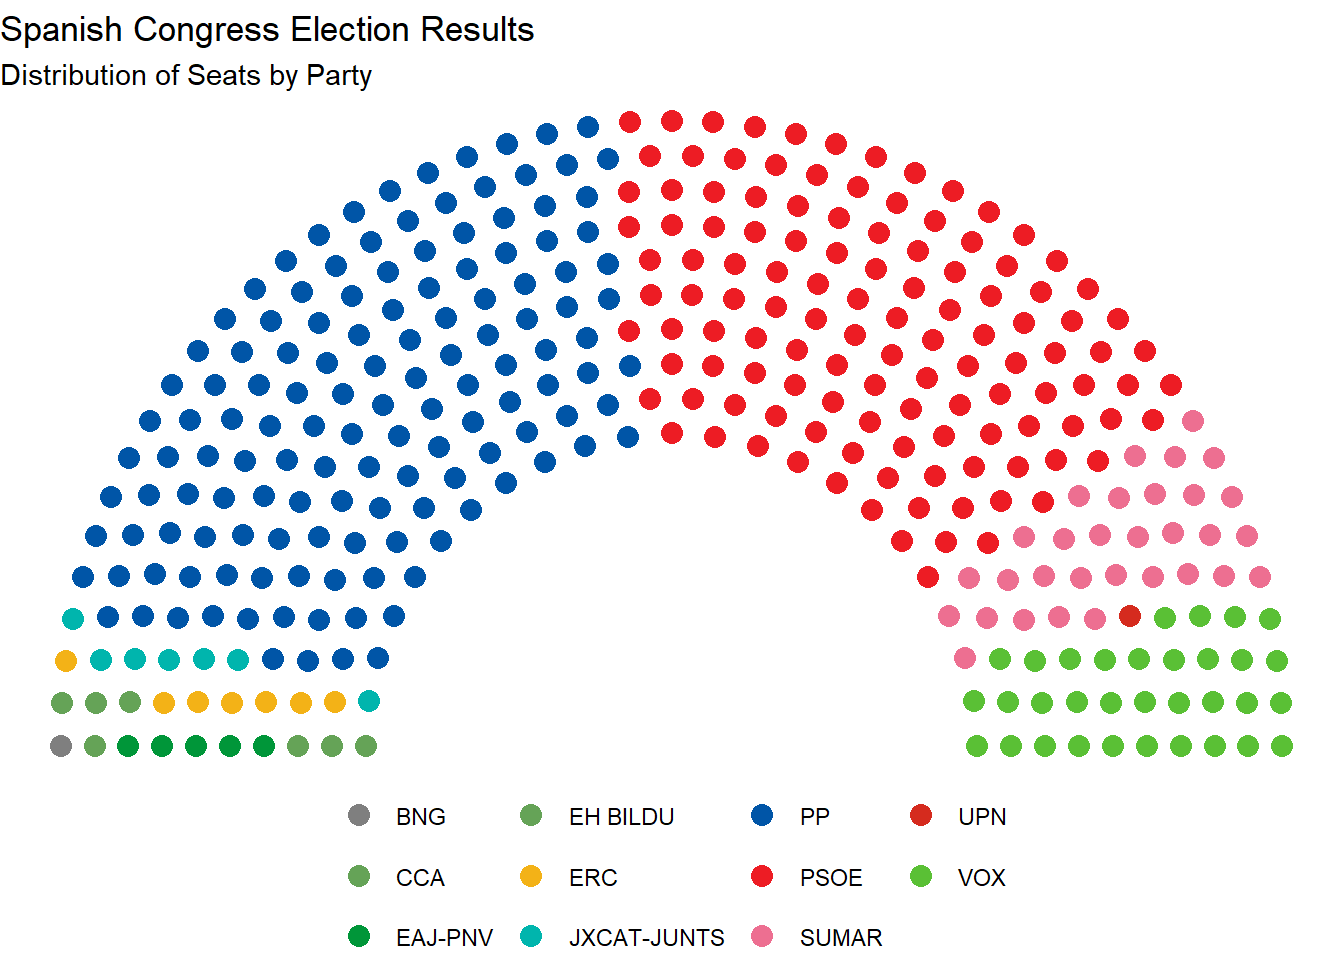
\includegraphics{Functionalities_files/figure-pdf/unnamed-chunk-23-1.pdf}

}

\end{figure}

\hypertarget{plot_parliament_distribution}{%
\subsubsection{\texorpdfstring{\texttt{plot\_parliament\_distribution}}{plot\_parliament\_distribution}}\label{plot_parliament_distribution}}

Generates a semicircle plot of parliamentary seat distribution using the
`ggparliament` package. It visualizes the number of seats allocated to
each party.

\begin{itemize}
\tightlist
\item
  \textbf{Inputs}: A data frame with seat distribution data.
\item
  \textbf{Outputs}: A \texttt{ggplot2} object representing the seat
  distribution in a semicircle plot.
\end{itemize}

\begin{quote}
\texttt{election\_data}: A data frame processed by the
\texttt{allocate\_seats\_dhondt()} function

\texttt{colors\_url}: A string URL pointing to the location of the RDA
file containing party colors. Default is set to
``https://github.com/mikadsr/Pollspain-data/raw/main/get\%20auxiliary\%20data/party\_colors\_hex.rda''.
\end{quote}

\begin{Shaded}
\begin{Highlighting}[]
\FunctionTok{plot\_parliament\_distribution}\NormalTok{(}\AttributeTok{election\_data =}\NormalTok{ final\_seat\_distribution)}
\end{Highlighting}
\end{Shaded}

\begin{figure}[H]

{\centering \includegraphics{Functionalities_files/figure-pdf/unnamed-chunk-24-1.pdf}

}

\end{figure}

\hypertarget{survey-data-1}{%
\subsection{Survey data}\label{survey-data-1}}

Calculates the average polling error for each polling firm and
party,based on the provided survey, election, and polling data. It
allows for optional filtering by specific polling firms and/or parties.

\begin{itemize}
\item
  \textbf{Inputs}: Two data frames: one for survey data and one for
  election results. Optional filters for polling firms and parties.
\item
  \textbf{Output:} a data frame with the average polling error for each
  polling firm and political party. It includes the date of the
  election, polling firm, political party, and the average polling
  error. With the option to filter based on the specified polling firms
  and/or parties if provided.
\end{itemize}

\begin{quote}
\texttt{survey\_data}: A data frame containing survey data with the
following columns:

\begin{itemize}
\tightlist
\item
  date\_elec: The date of the election.
\item
  polling\_firm: The name of the polling firm.
\item
  party: The political party for which the vote share is estimated.
\item
  vote\_share: The estimated vote share from the survey.
\end{itemize}

\texttt{election\_data}: A data frame obtained from
\texttt{get\_candidacy\_ballot\_data} containing election data with the
following columns:

\begin{itemize}
\tightlist
\item
  date\_elec: The date of the election.
\item
  abbrev\_candidacies: The abbreviation of the candidacies (parties).
\item
  total\_ballots: The total number of ballots cast for each party.
\end{itemize}

\texttt{poll\_data}: A data frame obtained from
\texttt{get\_poll\_station\_data()}containing polling data with the
following columns:

\begin{itemize}
\tightlist
\item
  date\_elec: The date of the election.
\item
  total\_ballots: The total number of ballots cast in each polling
  station.
\end{itemize}

\texttt{filter\_polling\_firm}: Optional. A vector of polling firms to
filter by. If NULL (default), no filtering by polling firm is applied.

\texttt{filter\_party}: Optional. A vector of parties to filter by. If
NULL (default), no filtering by party is applied.
\end{quote}

\begin{Shaded}
\begin{Highlighting}[]
\NormalTok{polling\_errors }\OtherTok{\textless{}{-}} \FunctionTok{calculate\_polling\_errors}\NormalTok{(}
  \AttributeTok{survey\_data =}\NormalTok{  survey\_data,}
  \AttributeTok{election\_data =}\NormalTok{ ballots\_data,}
  \AttributeTok{poll\_data =}\NormalTok{ poll\_station\_data)}
\end{Highlighting}
\end{Shaded}

\begin{Shaded}
\begin{Highlighting}[]
\FunctionTok{str}\NormalTok{(polling\_errors)}
\end{Highlighting}
\end{Shaded}

\begin{verbatim}
tibble [148 x 4] (S3: tbl_df/tbl/data.frame)
 $ date_elec        : Date[1:148], format: "2023-07-23" "2023-07-23" ...
 $ polling_firm     : chr [1:148] "40dB" "40dB" "40dB" "40dB" ...
 $ party            : chr [1:148] "PP" "PSOE" "SUMAR" "VOX" ...
 $ avg_polling_error: num [1:148] -1.757 6.04 5.092 1.996 0.331 ...
\end{verbatim}

\bookmarksetup{startatroot}

\hypertarget{testing-and-validation}{%
\chapter{Testing and Validation}\label{testing-and-validation}}

\bookmarksetup{startatroot}

\hypertarget{references}{%
\chapter*{References}\label{references}}
\addcontentsline{toc}{chapter}{References}

\markboth{References}{References}

\hypertarget{refs}{}
\begin{CSLReferences}{1}{0}
\leavevmode\vadjust pre{\hypertarget{ref-carolan2017open}{}}%
Carolan, L., \& Wolf, P. (2017). \emph{Open data in electoral
administration}. International IDEA. Retrieved from
\url{https://books.google.es/books?id=qk3XDwAAQBAJ}

\leavevmode\vadjust pre{\hypertarget{ref-pollspain2024}{}}%
DeSmedt, M. (2024). \emph{Pollspain-data}.
\url{https://github.com/mikadsr/Pollspain-data}.

\leavevmode\vadjust pre{\hypertarget{ref-europarl2019}{}}%
European Parliament. (2019). \emph{Understanding the d'hondt method}
(Briefing No. 637966). Brussels: European Parliament. Retrieved from
European Parliament website:
\url{https://www.europarl.europa.eu/RegData/etudes/BRIE/2019/637966/EPRS_BRI(2019)637966_EN.pdf}

\leavevmode\vadjust pre{\hypertarget{ref-INE_prov_Codes}{}}%
INE. (2024a). \emph{Código de provincia en españa}. Retrieved from
\url{https://ine.es/daco/daco42/codmun/cod_provincia.htm}

\leavevmode\vadjust pre{\hypertarget{ref-INE_MUN_Dictionary}{}}%
INE. (2024b). \emph{Diccionario de códigos de municipios en españa}.
Retrieved from
\url{https://ine.es/daco/daco42/codmun/diccionario24.xlsx}

\leavevmode\vadjust pre{\hypertarget{ref-interior2024}{}}%
Interior, M. del. (2024). \emph{Área de descargas - información
electoral}. Retrieved from
\url{https://infoelectoral.interior.gob.es/es/elecciones-celebradas/area-de-descargas/}

\leavevmode\vadjust pre{\hypertarget{ref-doi:10.1207ux2fs15506878jobem5002_1}{}}%
Kenski, K., \& Stroud, N. J. (2006). Connections between internet use
and political efficacy, knowledge, and participation. \emph{Journal of
Broadcasting \& Electronic Media}, \emph{50}(2), 173--192.
\url{https://doi.org/10.1207/s15506878jobem5002_1}

\leavevmode\vadjust pre{\hypertarget{ref-electionsBR}{}}%
Meireles, F., Silva, D., \& Costa, B. (2016). \emph{{electionsBR}: {R}
functions to download and clean {B}razilian electoral data}. Retrieved
from \url{http://electionsbr.com/}

\leavevmode\vadjust pre{\hypertarget{ref-perez2021}{}}%
Pérez, V., Aybar, C., \& Pavía, J. M. (2021). Spanish electoral archive.
SEA database. \emph{Scientific Data}, \emph{8}, 193.
\url{https://doi.org/10.1038/s41597-021-00975-y}

\leavevmode\vadjust pre{\hypertarget{ref-Schraff2022}{}}%
Schraff, D., Vergioglou, I., \& Demirci, B. B. (2022). The european
NUTS-level election dataset: A tool to map european electoral geography.
\emph{Party Politics}, \emph{29}, 570--579.
\url{https://doi.org/10.1177/13540688221083553}

\leavevmode\vadjust pre{\hypertarget{ref-wikipedia_espania_elections}{}}%
Wikipedia contributors. (2024a). Anexo: Elecciones en españa. Retrieved
from
\url{https://es.wikipedia.org/wiki/Anexo:Elecciones_en_Espa\%C3\%B1a}

\leavevmode\vadjust pre{\hypertarget{ref-wikipedia2024circunscripciones}{}}%
Wikipedia contributors. (2024b). \emph{Circunscripciones electorales del
congreso de los diputados}. Wikipedia, The Free Encyclopedia. Retrieved
from
\url{https://es.wikipedia.org/wiki/Circunscripciones_electorales_del_Congreso_de_los_Diputados}

\end{CSLReferences}



\printindex

\end{document}
